\documentclass[tikz,border=8pt]{standalone}
\usepackage{tikz}
\usepackage{amsmath}
\usetikzlibrary{shapes.geometric, arrows.meta, positioning, calc, fit, backgrounds}
%% qual-light-06 palette (cpt-city: ssz/qual-light-06, CC BY-SA 4.0)
\definecolor{qlBlue}{RGB}{182,206,229}
\definecolor{qlPink}{RGB}{229,181,197}
\definecolor{qlPeach}{RGB}{242,206,193}
\definecolor{qlYellow}{RGB}{249,235,170}
\definecolor{qlGreen}{RGB}{206,229,181}
\definecolor{qlTeal}{RGB}{182,228,209}
%% hue-matched darker accents for borders, phase bars, and arrows
\definecolor{qlBlueDk}{RGB}{60,96,140}
\definecolor{qlPeachDk}{RGB}{190,90,55}
\definecolor{qlGreenDk}{RGB}{86,140,64}
\definecolor{qlYellowDk}{RGB}{176,150,58}
\tikzset{
  mainbox/.style={rectangle, rounded corners=3pt, draw=qlBlueDk, fill=qlBlue,
    text width=5.2cm, align=center, font=\small\sffamily, inner sep=6pt, minimum height=1.1cm},
  excludebox/.style={rectangle, rounded corners=3pt, draw=qlPeachDk, fill=qlPeach,
    text width=6.2cm, align=left, font=\small\sffamily, inner sep=6pt},
  phasebox/.style={rectangle, rounded corners=3pt, draw=qlBlueDk, fill=qlBlueDk,
    text=white, font=\small\bfseries\sffamily, align=center, inner sep=5pt,
    minimum width=2.0cm, minimum height=2.8cm, rotate=90},
  sourcebox/.style={rectangle, rounded corners=3pt, draw=qlYellowDk, fill=qlYellow,
    text width=5.2cm, align=center, font=\small\sffamily, inner sep=6pt, minimum height=1.1cm},
  includedbox/.style={rectangle, rounded corners=3pt, draw=qlGreenDk, fill=qlGreen,
    text width=5.2cm, align=center, font=\small\bfseries\sffamily, inner sep=6pt, minimum height=1.1cm},
  arrow/.style={-Stealth, thick, color=qlBlueDk},
  darrow/.style={-Stealth, thick, color=qlPeachDk, dashed},
}

\begin{document}
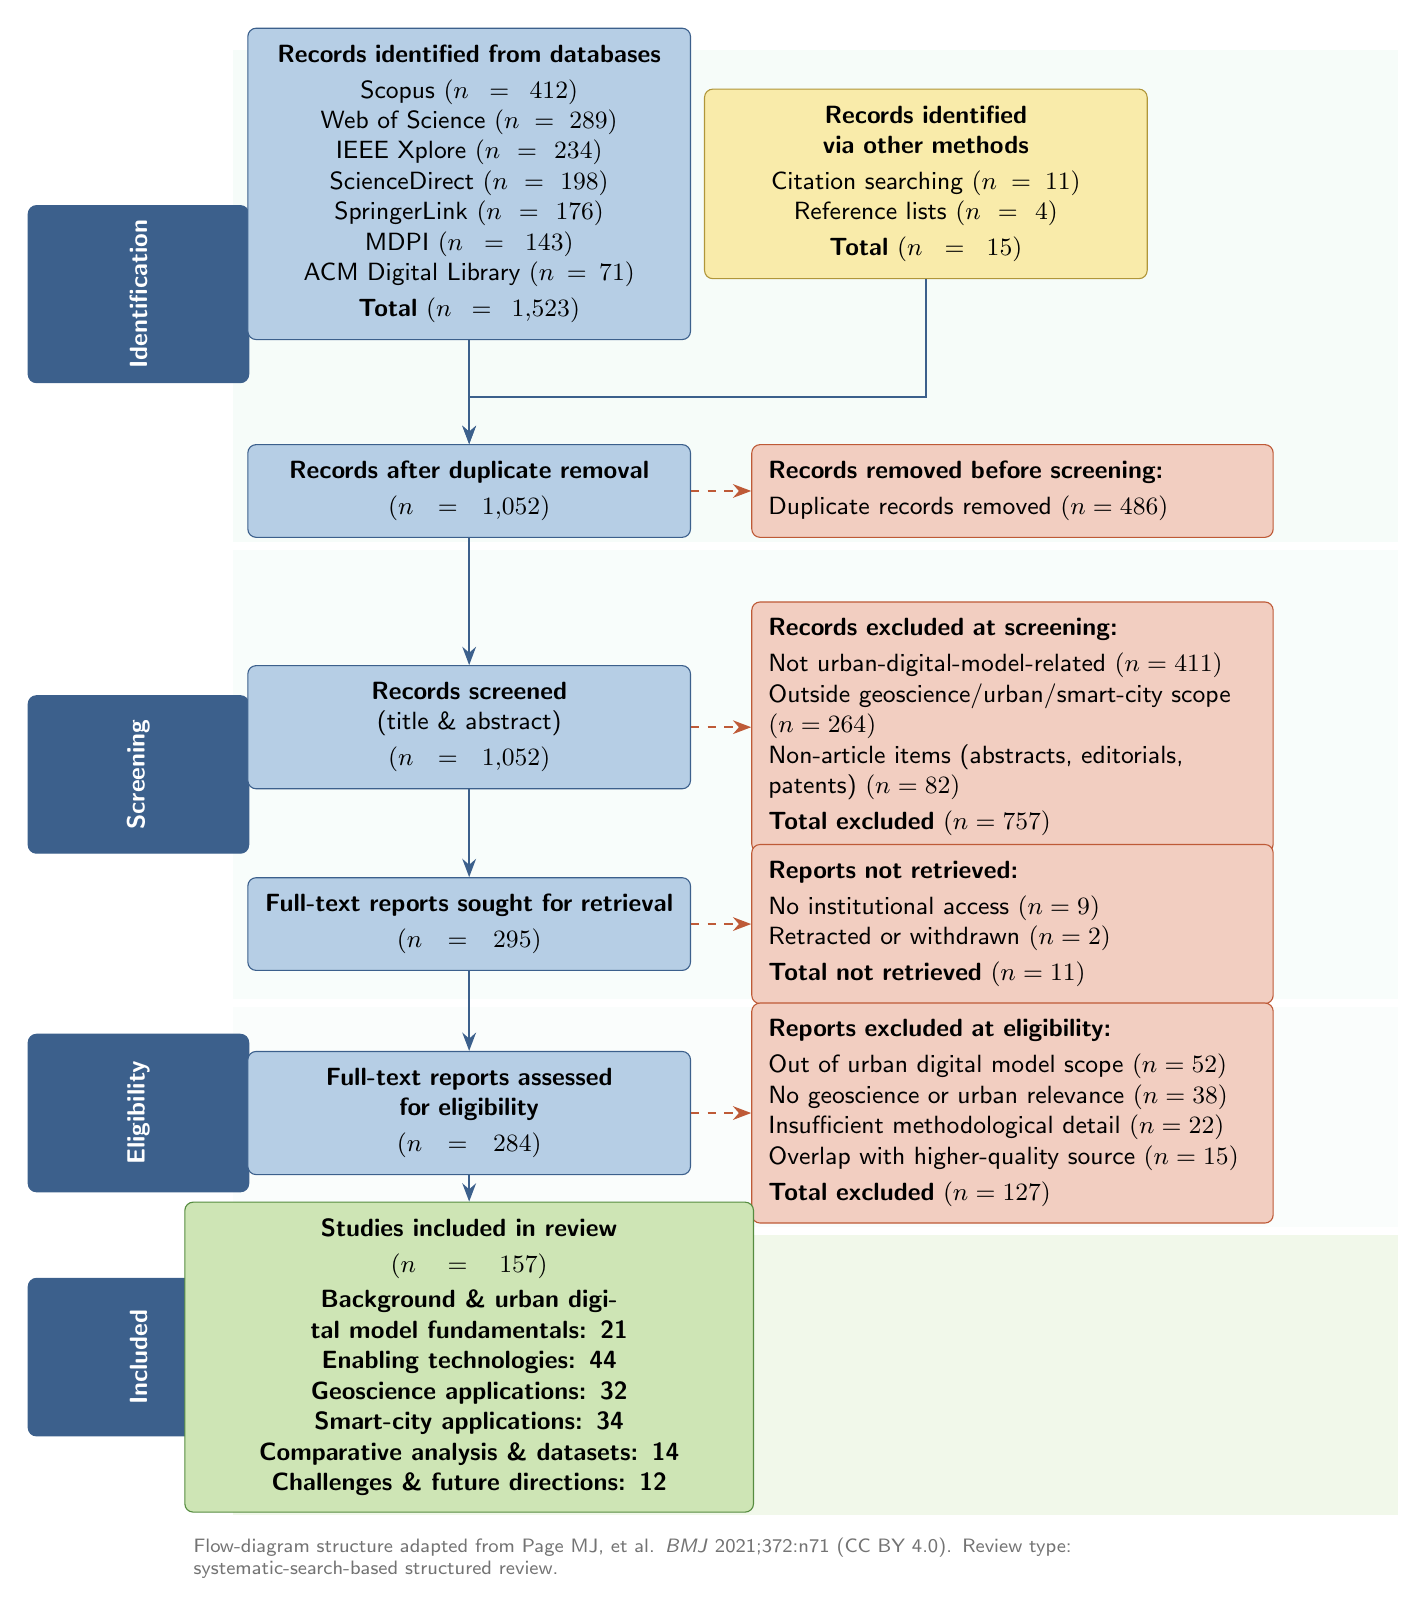
\begin{tikzpicture}[node distance=0.55cm and 1.2cm]

%% PHASE LABELS
\node[phasebox] (id_label) at (-1.2, -1.4)  {Identification};
\node[phasebox] (sc_label) at (-1.2, -7.5)  {Screening};
\node[phasebox] (el_label) at (-1.2, -11.8) {Eligibility};
\node[phasebox] (in_label) at (-1.2, -14.9) {Included};

%% IDENTIFICATION
\node[mainbox] (db_search) at (3.0, 0)
  {\textbf{Records identified from databases}\\[2pt]
   Scopus $(n = 412)$\\
   Web of Science $(n = 289)$\\
   IEEE Xplore $(n = 234)$\\
   ScienceDirect $(n = 198)$\\
   SpringerLink $(n = 176)$\\
   MDPI $(n = 143)$\\
   ACM Digital Library $(n = 71)$\\[2pt]
   \textbf{Total} $(n = 1{,}523)$};

\node[sourcebox] (other_search) at (8.8, 0)
  {\textbf{Records identified via other methods}\\[2pt]
   Citation searching $(n = 11)$\\
   Reference lists $(n = 4)$\\[2pt]
   \textbf{Total} $(n = 15)$};

%% exclusion (red) boxes: each vertically centred on its source box (so the
%% dashed arrows are exactly horizontal), placed to the right with a clear gap
\node[excludebox] (duplicates) at (9.9, -3.9)
  {\textbf{Records removed before screening:}\\[2pt]
   Duplicate records removed $(n = 486)$};

\node[excludebox] (excluded_screen) at (9.9, -6.9)
  {\textbf{Records excluded at screening:}\\[2pt]
   Not urban-digital-model-related $(n = 411)$\\
   Outside geoscience/urban/smart-city scope $(n = 264)$\\
   Non-article items (abstracts, editorials, patents) $(n = 82)$\\[2pt]
   \textbf{Total excluded} $(n = 757)$};

\node[excludebox] (not_retrieved) at (9.9, -9.4)
  {\textbf{Reports not retrieved:}\\[2pt]
   No institutional access $(n = 9)$\\
   Retracted or withdrawn $(n = 2)$\\[2pt]
   \textbf{Total not retrieved} $(n = 11)$};

\node[excludebox] (excluded_elig) at (9.9, -11.8)
  {\textbf{Reports excluded at eligibility:}\\[2pt]
   Out of urban digital model scope $(n = 52)$\\
   No geoscience or urban relevance $(n = 38)$\\
   Insufficient methodological detail $(n = 22)$\\
   Overlap with higher-quality source $(n = 15)$\\[2pt]
   \textbf{Total excluded} $(n = 127)$};

\node[mainbox] (records_id) at (3.0, -3.9)
  {\textbf{Records after duplicate removal}\\[2pt]
   $(n = 1{,}052)$};

%% SCREENING
\node[mainbox] (screened) at (3.0, -6.9)
  {\textbf{Records screened}\\
   (title \& abstract)\\[2pt]
   $(n = 1{,}052)$};

\node[mainbox] (sought) at (3.0, -9.4)
  {\textbf{Full-text reports sought for retrieval}\\[2pt]
   $(n = 295)$};

%% ELIGIBILITY
\node[mainbox] (assessed) at (3.0, -11.8)
  {\textbf{Full-text reports assessed}\\
   \textbf{for eligibility}\\[2pt]
   $(n = 284)$};

%% INCLUDED
\node[includedbox, text width=6.8cm] (included) at (3.0, -14.9)
  {\textbf{Studies included in review}\\[2pt]
   $(n = 157)$\\[2pt]
   \small Background \& urban digital model fundamentals: 21\\
   \small Enabling technologies: 44\\
   \small Geoscience applications: 32\\
   \small Smart-city applications: 34\\
   \small Comparative analysis \& datasets: 14\\
   \small Challenges \& future directions: 12};

%% ARROWS -- main flow (both identification boxes merge below db_search,
%% so no line crosses the "Records identified from databases" box)
\draw[arrow] (db_search.south) -- (records_id.north);
\draw[arrow] (other_search.south) |- ($(records_id.north)+(0,0.6)$) -- (records_id.north);
\draw[arrow] (records_id.south) -- (screened.north);
\draw[arrow] (screened.south)   -- (sought.north);
\draw[arrow] (sought.south)     -- (assessed.north);
\draw[arrow] (assessed.south)   -- (included.north);

%% ARROWS -- exclusion branches (each strictly horizontal: source and target
%% share the same y, so no rotation)
\draw[darrow] (records_id.east) -- (duplicates.west);
\draw[darrow] (screened.east)   -- (excluded_screen.west);
\draw[darrow] (sought.east)     -- (not_retrieved.west);
\draw[darrow] (assessed.east)   -- (excluded_elig.west);

%% BACKGROUND BANDS
\begin{pgfonlayer}{background}
  \fill[qlTeal, opacity=0.12] (-0.0, 1.7)   rectangle (14.8, -4.55);
  \fill[qlTeal, opacity=0.09] (-0.0, -4.65) rectangle (14.8, -10.35);
  \fill[qlTeal, opacity=0.07] (-0.0, -10.45) rectangle (14.8, -13.25);
  \fill[qlGreen, opacity=0.28] (-0.0, -13.35) rectangle (14.8, -16.9);
\end{pgfonlayer}

\node[font=\scriptsize\sffamily\color{black!55}, align=left, text width=12cm]
  at (5.5, -17.45)
  {Flow-diagram structure adapted from Page MJ, et al. \textit{BMJ} 2021;372:n71 (CC BY 4.0).
   Review type: systematic-search-based structured review.};

\end{tikzpicture}
\end{document}
